%-----------------------------------
% Kapitel 4: Soll-Konzeption des KI-gestützten Incident-Management-Prozesses
%-----------------------------------
\section{Soll-Konzeption des KI-gestützten Incident-Management-Prozesses}
\label{sollKonzeption}

Kapitel~\ref{sollKonzeption} tritt in die Redesign-Phase des in Abschnitt~\ref{bpmnDigitalisierung} beschriebenen Lebenszyklus ein und entwickelt auf Grundlage der drei in Abschnitt~\ref{schwachstellen} abgeleiteten Automatisierungspotenziale jenes Artefakt, das Abschnitt~\ref{methodik} als Ziel des gestaltungsorientierten Vorgehens benennt. Die Konzeption ist durchgehend hybrid angelegt. Automatisiert wird dort, wo dies fachlich tragf\"ahig ist; die Entscheidung verbleibt beim Menschen, wo Qualit\"at, Recht oder Akzeptanz es verlangen.

\subsection{Prämissen und Anforderungen an den hybriden Workflow}
\label{praemissen}

Bevor die einzelnen KI-gest\"utzten Schritte entwickelt werden, sind die Bedingungen festzulegen, unter denen sie arbeiten. Dazu z\"ahlen die technischen, organisatorischen und rechtlichen Voraussetzungen, die Abschnitt~\ref{voraussetzungen} als Design-Pr\"amissen ableitet, sowie das Prinzip der menschlichen Beteiligung, das Abschnitt~\ref{hitl} begr\"undet.

\subsubsection{Technische und organisatorische Voraussetzungen (inkl. DSGVO und EU AI Act als Design-Prämissen)}
\label{voraussetzungen}

Die KI-Komponenten erg\"anzen das bestehende System, statt an seine Stelle zu treten. Das ITSM-Tool bleibt f\"uhrendes System f\"ur Tickets, Status und Historie, w\"ahrend die Modelle \"uber Schnittstellen darauf zugreifen und ihre Ergebnisse als Vorschlagsfelder in den Vorgang zur\"uckschreiben. Inhaltliche Grundlage maschineller L\"osungsvorschl\"age sind die Wissens- und die Known-Error-Datenbank, deren Pflegezustand die Qualit\"at der Ausgaben unmittelbar begrenzt; wie der Zugriff technisch erfolgt, behandelt Abschnitt~\ref{loesungsvorschlaege}. Eine dritte Voraussetzung betrifft das Betriebsmodell. Ob das Modell im eigenen Rechenzentrum oder in einer Cloud-Umgebung innerhalb der Europ\"aischen Union l\"auft, bestimmt, welche Daten das Unternehmen verlassen, und ist damit bereits eine datenschutzrechtliche Weichenstellung.

Organisatorisch setzt der Betrieb eine gekl\"arte Prozessverantwortung voraus. Die ISO/IEC~20000-1 verlangt ein dokumentiertes Service-Management-System mit festgelegten Rollen, Zielen und Steuerungsmechanismen, in das sich ein KI-gest\"utzter Ablauf einf\"ugen muss.\footcite[Vgl.][Abschn.~4.4, 5.3, 6.2 und 9.1]{ISO20000} Iden und Eikebrokk arbeiten in einer systematischen Literaturauswertung Erfolgsfaktoren von ITSM-Einf\"uhrungen heraus, unter denen die Unterst\"utzung durch das Management, die Schulung der Beteiligten sowie Kommunikation und Organisationskultur wiederkehrend genannt w\"urden.\footcite[Vgl.][hier S.~518]{IdenEikebrokk2013} Da auch hier eine eingespielte Arbeitsweise ver\"andert wird, sieht die Konzeption zus\"atzlich vor, den Prozess stufenweise aktivierbar zu gestalten und den Automatisierungsgrad erst mit belegter Vorschlagsqualit\"at zu erh\"ohen; dies entspricht dem ITIL-Leitprinzip eines iterativen Vorgehens mit R\"uckmeldung.\footcite[Vgl.][S.~30]{Agutter2020}

Tickets enthalten personenbezogene Daten, unter Umst\"anden auch solche besonderer Kategorien im Sinne des Art.~9 Abs.~1 DSGVO.\footcite[Vgl.][Art.~9 Abs.~1]{DSGVO} Neben der Identit\"at des Melders enth\"alt der Freitext gelegentlich Angaben, die auf gesundheitliche oder arbeitsrechtliche Sachverhalte schlie{\ss}en lassen. Aus den Grunds\"atzen der Datenschutz-Grundverordnung folgt zun\"achst, dass nur die f\"ur die St\"orungsbearbeitung erforderlichen Daten an ein Modell \"ubergeben werden d\"urfen und eine Weiterverwendung zu anderen Zwecken, etwa zur Leistungskontrolle einzelner Agenten, ausscheidet.\footcite[Vgl.][Art.~5 Abs.~1 lit.~b und c]{DSGVO} Der Datenschutz durch Technikgestaltung verlangt, solche Vorkehrungen bereits in der Architektur vorzusehen.\footcite[Vgl.][Art.~25 Abs.~1]{DSGVO} Hinzu treten die Anforderungen an die Sicherheit der Verarbeitung\footcite[Vgl.][Art.~32]{DSGVO} sowie die Pr\"ufung, ob der Einsatz eine Datenschutz-Folgenabsch\"atzung erfordert.\footcite[Vgl.][Art.~35 Abs.~1]{DSGVO} F\"ur die Prozessgestaltung am folgenreichsten ist Art.~22 Abs.~1 DSGVO, der das Recht gew\"ahrt, nicht einer ausschlie{\ss}lich auf automatisierter Verarbeitung beruhenden Entscheidung unterworfen zu werden, die rechtliche Wirkung entfaltet oder in \"ahnlicher Weise erheblich beeintr\"achtigt.\footcite[Vgl.][Art.~22 Abs.~1]{DSGVO} Bei der \"uberwiegenden Zahl der Support-Vorg\"ange d\"urfte die Vorschrift nicht einschl\"agig sein, da die Zuordnung einer Ticketkategorie niemanden erheblich beeintr\"achtigt. Wann eine Entscheidung in \"ahnlicher Weise erheblich beeintr\"achtigt, konkretisiert die Artikel-29-Datenschutzgruppe dahin, dass sie auf die Umst\"ande oder das Verhalten der betroffenen Person sp\"urbar einwirken oder sie \"uber l\"angere Zeit benachteiligen muss.\footcite[Vgl.][S.~21]{WP29Leitlinien2018} Gemessen daran l\"asst sich eine erhebliche Wirkung dort nicht ausschlie{\ss}en, wo ein Vorgang ohne menschliche Beteiligung abgewiesen oder geschlossen wird und der Melder infolgedessen arbeitsunf\"ahig bleibt. Der Soll-Prozess sieht deshalb vor, abschlie{\ss}ende Entscheidungen \"uber Tickets mit erheblicher Tragweite nicht vollautomatisiert zu treffen. Der Europ\"aische Datenschutzausschuss hebt erg\"anzend hervor, die Verantwortlichkeit verbleibe beim einsetzenden Unternehmen und die Rechtsgrundlage sei f\"ur jede Verarbeitungsphase gesondert zu pr\"ufen.\footcite[Vgl.][S.~20]{EDSA2024}

Die KI-Verordnung folgt einem risikobasierten Ansatz und kn\"upft die Pflichten an die Einstufung des jeweiligen Systems. Zugrunde gelegt wird die Fassung, die sie durch die am 27.~Juli 2026 in Kraft getretene Digital-Omnibus-Verordnung zur KI erhalten hat.\footcite[Vgl.][Art.~4]{KIVO2026} Ein interner Assistent, der Support-Agenten Kategorien, Priorit\"aten und L\"osungswege vorschl\"agt, ist nach der hier vertretenen Einsch\"atzung regelm\"a{\ss}ig nicht als Hochrisiko-System einzuordnen, da er weder \"uber den Zugang zu Besch\"aftigung oder wesentlichen Diensten entscheidet noch Besch\"aftigte beobachtet oder bewertet. Diese Einsch\"atzung steht allerdings unter einem Vorbehalt, denn Anhang~III Nr.~4 lit.~b der Verordnung erfasst Systeme, die f\"ur die Zuweisung von Aufgaben aufgrund des individuellen Verhaltens oder pers\"onlicher Merkmale oder Eigenschaften oder f\"ur die Beobachtung und Bewertung der Leistung und des Verhaltens von Besch\"aftigten verwendet werden sollen.\footcite[Vgl.][Anhang~III Nr.~4 lit.~b]{KIVO} Die Weiterleitung eines Tickets an eine Bearbeitungsgruppe weist zwar Arbeit zu, kn\"upft im Konzept aber allein an Merkmale des Tickets und an Zust\"andigkeitsgruppen an und nicht an Verhalten oder Merkmale einzelner Bearbeiter. Die in Abschnitt~\ref{kategorisierungSoll} vorgesehene Protokollierung jeder Agentenkorrektur ber\"uhrt den Tatbestand dagegen dem Wortlaut nach. Ausschlaggebend ist die Zweckbindung: Die Protokolle dienen der Nachjustierung des Kategorisierungsmodells und der \"Uberpr\"ufung des Schwellenwerts, nicht der Beurteilung einzelner Besch\"aftigter. Der Entwurf sieht deshalb vor, die Korrekturdaten ausschlie{\ss}lich aggregiert auszuwerten und eine personenbezogene Leistungsbewertung auszuschlie{\ss}en. Unterbleibt diese Festlegung, verschiebt sich die Einstufung, und die Pflichten f\"ur Hochrisiko-Systeme greifen.

Selbst wenn ein System einen Bereich des Anhangs~III ber\"uhrt, gilt es nicht als hochriskant, sofern es kein erhebliches Risiko birgt, etwa weil es lediglich eine eng gefasste Verfahrensaufgabe oder eine vorbereitende Aufgabe f\"ur eine Bewertung durchf\"uhrt; ausgenommen bleibt jedes System, das ein Profiling nat\"urlicher Personen vornimmt.\footcite[Vgl.][Art.~6 Abs.~3]{KIVO} Diese Einsch\"atzung hat der Anbieter vor dem Inverkehrbringen oder der Inbetriebnahme zu dokumentieren.\footcite[Vgl.][Art.~6 Abs.~4]{KIVO} Die menschlichen Entscheidungsknoten des Soll-Prozesses st\"utzen diese Einordnung, da die Vorschl\"age des Systems eine Entscheidung des Agenten vorbereiten und nicht ersetzen. Einschl\"agig bleibt gleichwohl die Transparenzpflicht, nach der Anbieter ein System, das f\"ur die direkte Interaktion mit nat\"urlichen Personen bestimmt ist, so zu konzipieren haben, dass diese dar\"uber informiert werden, dass sie mit einem KI-System interagieren; bei einer Eigenentwicklung trifft diese Pflicht das Unternehmen selbst.\footcite[Vgl.][Art.~50 Abs.~1]{KIVO}

Unabh\"angig von der Einstufung gilt zudem Art.~4 der KI-Verordnung, nach dem der Betreiber Ma{\ss}nahmen ergreift, um die KI-Kompetenz der mit dem System befassten Personen zu f\"ordern; ein bestimmtes Kompetenzniveau schreibt die Vorschrift seit der \"Anderung nicht mehr vor.\footcites[Vgl.][Art.~4]{KIVO}[][Art.~1 Nr.~5]{KIVO2026} Das deckt sich mit dem Schulungsbedarf, den Abschnitt~\ref{herausforderungen} aus der Akzeptanzbetrachtung ableitet. Die Anforderungen an die menschliche Aufsicht gelten demgegen\"uber nur f\"ur Hochrisiko-Systeme verbindlich;\footcite[Vgl.][Art.~14]{KIVO} f\"ur Systeme nach Anhang~III sind diese Pflichten infolge der \"Anderungsverordnung erst ab dem 2.~Dezember 2027 anzuwenden.\footcite[Vgl.][Art.~1 Nr.~40]{KIVO2026} Der Entwurf \"ubernimmt sie dennoch als Gestaltungsleitlinie des Soll-Prozesses. Diese \"Ubernahme ist eine bewusste Design-Entscheidung und keine Rechtspflicht; die dort genannten Anforderungen an Verst\"andlichkeit, Eingriffsm\"oglichkeit und kritische Pr\"ufung tragen unabh\"angig von der Einstufung zur Qualit\"atssicherung bei.

Neben dem Datenschutz- und dem Produktrecht ist das Betriebsverfassungsrecht zu ber\"ucksichtigen. Nach \S~87 Abs.~1 Nr.~6 BetrVG unterliegt die Einf\"uhrung und Anwendung technischer Einrichtungen, die dazu bestimmt sind, das Verhalten oder die Leistung der Arbeitnehmer zu \"uberwachen, der Mitbestimmung des Betriebsrats.\footcite[Vgl.][\S~87 Abs.~1 Nr.~6]{BetrVG} Ein System, das jede Korrektur eines Agenten protokolliert und diese Protokolle auswertbar vorh\"alt, erzeugt Verhaltens- und Leistungsdaten. Es handelt sich dabei um Besch\"aftigtendaten, f\"ur die Art.~88 Abs.~1 DSGVO den Mitgliedstaaten eigene Regelungen er\"offnet;\footcite[Vgl.][Art.~88 Abs.~1]{DSGVO} in Deutschland f\"ullt \S~26 BDSG diese \"Offnungsklausel aus und l\"asst insbesondere Kollektivvereinbarungen als Rechtsgrundlage zu.\footcite[Vgl.][\S~26]{BDSG} Nach der Rechtsprechung des Gerichtshofs der Europ\"aischen Union (EuGH) sind solche Regelungen allerdings nur dann als spezifischere Vorschriften anzuerkennen, wenn sie die Anforderungen des Art.~88 Abs.~2 DSGVO erf\"ullen.\footcites[Vgl.][Art.~88 Abs.~2]{DSGVO}[][Rn.~74\,f.]{EuGH2023} Eine Betriebsvereinbarung, die ihrerseits geeignete und besondere Ma{\ss}nahmen zur Wahrung der menschlichen W\"urde, der berechtigten Interessen und der Grundrechte der Besch\"aftigten vorsieht, kann die Verarbeitung damit zugleich datenschutz- und betriebsverfassungsrechtlich tragen. Ob der Mitbestimmungstatbestand im Einzelfall er\"offnet ist, bleibt einer arbeitsrechtlichen Pr\"ufung vorbehalten, die nicht Gegenstand dieser Arbeit ist. F\"ur die Gestaltung folgt daraus gleichwohl, den Betriebsrat fr\"uhzeitig einzubeziehen und Zweck, Aufbewahrungsdauer und Auswertungsform der Korrekturprotokolle in einer Betriebsvereinbarung festzuschreiben. Diese Festlegung tr\"agt zugleich zu der in Abschnitt~\ref{herausforderungen} behandelten Akzeptanz bei, da andernfalls der Verdacht einer Leistungskontrolle im Raum bliebe.

Die genannten Rechtsakte weisen damit in dieselbe Gestaltungsrichtung. Maschinelle Vorarbeit ist zul\"assig, die Letztentscheidung an kritischen Punkten bleibt beim Menschen.

\subsubsection{Das Konzept des \glqq Human-in-the-Loop\grqq{}}
\label{hitl}

Das Konzept des Human-in-the-Loop (HITL) beschreibt Ans\"atze, in denen Mensch und lernendes System innerhalb eines Arbeits- oder Entscheidungsprozesses zusammenwirken, statt einander abzul\"osen. Mosqueira-Rey et al.~ordnen die vorliegenden Auspr\"agungen in einer \"Ubersicht und unterscheiden dabei Active Learning, bei dem das System gezielt nach Annotationen verlange, Interactive Machine Learning mit fortlaufender R\"uckkopplung w\"ahrend des Lernvorgangs sowie Machine Teaching, bei dem Fachexperten ihr Wissen strukturiert einbr\"achten.\footcite[Vgl.][hier S.~3006]{MosqueiraRey2023} Diese Varianten setzen \"uberwiegend am Training der Modelle an. Die vorliegende Arbeit verwendet den Begriff enger und bezieht ihn auf die Entscheidungsteilhabe im laufenden Betrieb.

Auf die Prozessgestaltung \"ubertragen bedeutet HITL, dass das Modell Vorschl\"age erzeugt und der Mensch \"uber deren Verwendung entscheidet. Die vorliegende Konzeption setzt diese Beteiligung allerdings nicht auf einer einheitlichen Stufe an, sondern staffelt sie nach der Verl\"asslichkeit des Vorschlags. Unterhalb des in Abschnitt~\ref{fallback} begr\"undeten Konfidenzschwellenwerts ist die menschliche Entscheidung ein eigener und zwingender Prozessschritt, denn der Agent bestimmt Kategorie und Priorit\"at, bevor der Vorgang fortschreitet; diese Auspr\"agung wird im Folgenden als Human-in-the-Loop im engeren Sinne bezeichnet. Oberhalb des Schwellenwerts \"ubernimmt der Prozess den Vorschlag vorl\"aufig, ohne einen gesonderten Pr\"ufschritt einzuf\"ugen, w\"ahrend der Agent, der den Vorgang auf dem assistierten Pfad ohnehin bearbeitet, die vorbelegten Felder samt Konfidenzangabe vor sich hat und jederzeit \"andern kann; diese Auspr\"agung wird im Folgenden als Human-on-the-Loop bezeichnet. Beide Bezeichnungen dienen als Arbeitsbegriffe dieser Arbeit; sie kn\"upfen an die gebr\"auchliche Unterscheidung von Autonomiestufen an, ohne einer bestimmten Systematik zu folgen. Der Unterschied liegt mithin darin, ob die Handlung des Menschen den Ablauf anh\"alt. Die Rollenverteilung bleibt in beiden F\"allen eindeutig, denn das Modell wirkt als Assistenzsystem und der Mensch als Entscheidungsinstanz. Zugleich entsteht aus jeder Korrektur eine dokumentierte Abweichung, die sich sp\"ater zur Bewertung der Vorschlagsqualit\"at auswerten l\"asst. Vollst\"andig ohne menschliche Beteiligung l\"auft allein der Self-Service-Pfad f\"ur den in Abschnitt~\ref{loesungsvorschlaege} festgelegten Katalog risikoarmer Standardf\"alle; seine Abgrenzung folgt unmittelbar den rechtlichen Pr\"amissen aus Abschnitt~\ref{voraussetzungen}.

Die Beteiligung des Menschen erf\"ullt ihren Zweck allerdings nur, wenn sie \"uber eine formale Best\"atigung hinausgeht. Die Artikel-29-Datenschutzgruppe h\"alt in ihren Leitlinien fest, eine Aufsicht sei nur dann beachtlich, wenn sie durch eine Person mit entsprechender Befugnis und Kompetenz erfolge, die die Entscheidung tats\"achlich \"uberpr\"ufe und dabei \"uber alle relevanten Informationen verf\"uge; eine routinem\"a{\ss}ige \"Ubernahme des maschinellen Ergebnisses gen\"uge nicht.\footcite[Vgl.][S.~22]{WP29Leitlinien2018} Daraus folgt eine praktische Anforderung an die Gestaltung. Werden Agenten an einer Kennzahl gemessen, die kurze Bearbeitungszeiten belohnt, entsteht ein Anreiz, Vorschl\"age ungepr\"uft zu \"ubernehmen; der Prozess liefe dann faktisch vollautomatisiert ab, ohne dass dies im Modell sichtbar w\"urde.

Wie die Entscheidungsknoten auszugestalten sind, l\"asst sich an validierten Leitlinien der Mensch-KI-Interaktion ausrichten. Amershi et al.~empfehlen unter anderem, den Nutzern deutlich zu machen, was das System leisten kann und wo seine Grenzen liegen, die Unsicherheit einer Ausgabe erkennbar zu halten, effiziente Korrekturm\"oglichkeiten vorzusehen und das Systemverhalten nachvollziehbar zu erl\"autern.\footcite[Vgl.][hier S.~3]{Amershi2019} F\"ur den Soll-Prozess bedeutet dies, einen Vorschlag nicht als feststehendes Ergebnis, sondern mit einem Hinweis auf seine Verl\"asslichkeit darzustellen und die Korrektur mit nicht mehr Aufwand zu belegen als die Best\"atigung. Abschnitt~\ref{entscheidungsknoten} greift diese Anforderungen bei der Definition der maschinellen und menschlichen Entscheidungsknoten auf.

\subsection{Entwicklung der KI-gestützten Prozessschritte}
\label{prozessschritte}

Die folgenden Abschnitte setzen die drei in Abschnitt~\ref{schwachstellen} abgeleiteten Potenziale in derselben Reihenfolge um. Sie bauen aufeinander auf, denn eine strukturierte Erfassung schafft erst die Grundlage f\"ur eine verl\"assliche Kategorisierung, und beide zusammen bilden die Voraussetzung f\"ur brauchbare L\"osungsvorschl\"age. \autoref{fig:prozessschritte} zeigt, wie die drei Schritte ineinandergreifen.

\begin{figure}[htbp]
	\centering
	\caption{Zusammenspiel der drei KI-gest\"utzten Prozessschritte}
	\label{fig:prozessschritte}
	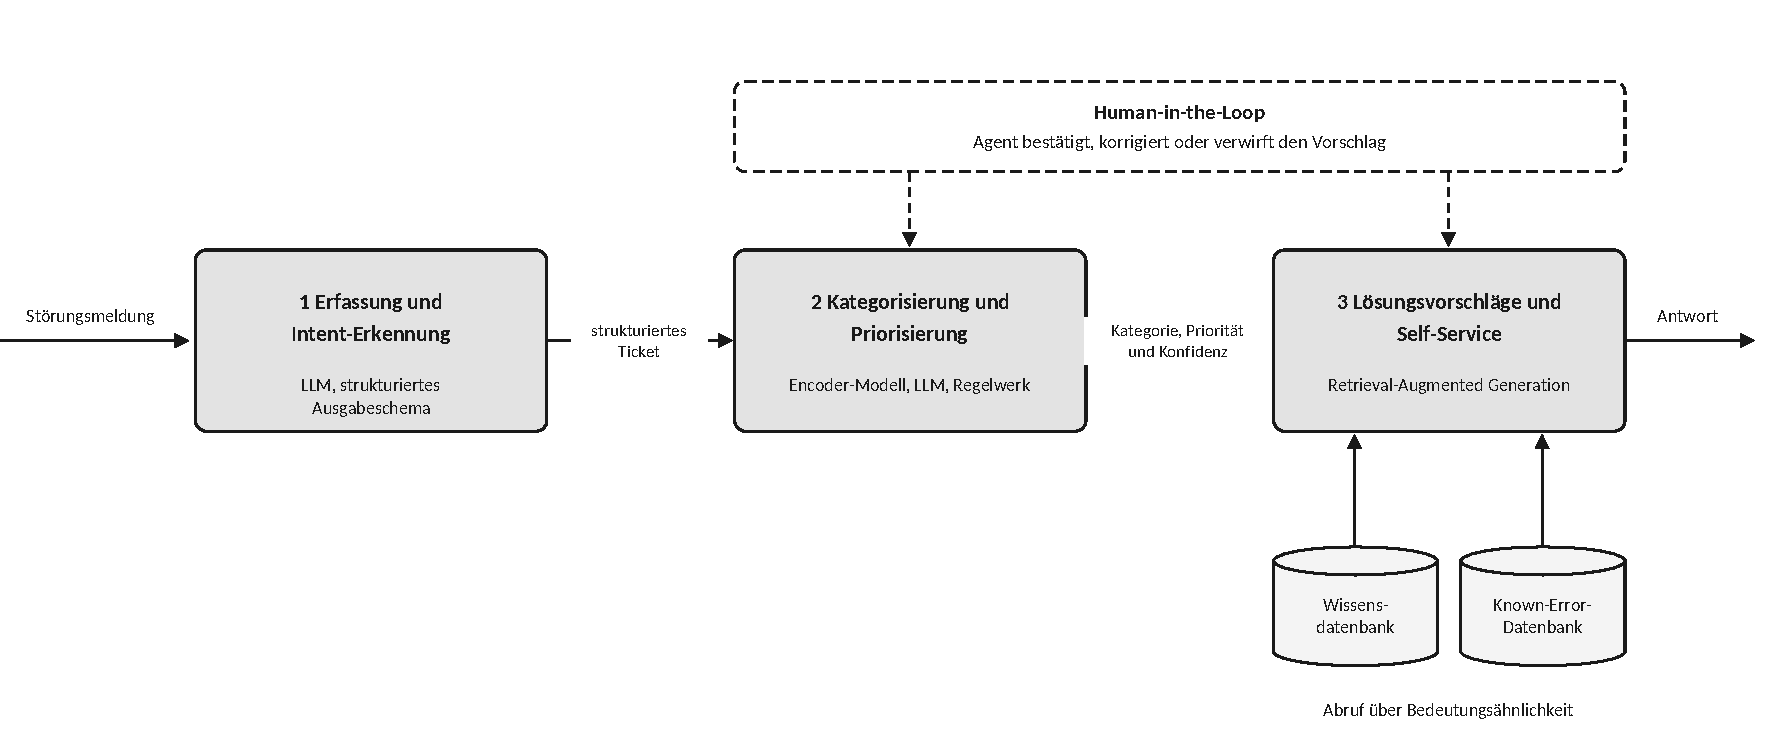
\includegraphics[width=\textwidth]{abb/abb6-ki-prozessschritte.pdf}
\end{figure}

\subsubsection{Automatisierte Ticketerfassung und Intent-Erkennung durch LLMs}
\label{ticketerfassung}

Am Prozessbeginn tritt an die Stelle des starren Formulars ein dialogorientierter Zugang. Der Anwender schildert die St\"orung \"uber Portal oder Chat in eigenen Worten, w\"ahrend ein LLM aus dem Freitext die strukturierten Kernangaben gewinnt, also den betroffenen Service, das beobachtete Symptom, den Wortlaut einer Fehlermeldung, den Zeitpunkt des Auftretens sowie Hinweise auf Dringlichkeit und Reichweite. Parallel dazu bestimmt das Modell das Anliegen. Besonderes Gewicht hat dabei die Unterscheidung zwischen Incident und Service Request, weil sie nach der in Abschnitt~\ref{itilEinordnung} dargelegten Begrifflichkeit \"uber den weiteren Prozesspfad entscheidet. Telefonische Meldungen bleiben davon unber\"uhrt; sie erreichen weiterhin den Agenten, der den Dialog stellvertretend f\"uhrt. Abschnitt~\ref{prozessarchitektur} bildet diesen Kanal als eigenen Prozesseintritt ab.

Die Erkennung des Anliegens l\"asst sich als Klassifikationsaufgabe formulieren. Parikh et al.~untersuchen Zero- und Few-Shot-Verfahren zur Intent-Klassifikation und zeigen, dass brauchbare Ergebnisse ohne einen umfangreichen Bestand von Hand zugeordneter Beispiele erreichbar seien.\footcite[Vgl.][hier S.~744\,f.]{Parikh2023} F\"ur den Support ist das von Belang, weil ein neu aufgesetzter Intent-Katalog andernfalls \"uber Monate hinweg zun\"achst Trainingsmaterial sammeln m\"usste. Die Steuerung erfolgt \"uber Prompts, also Anweisungen, die dem Modell die Aufgabe vorgeben, ohne seine Parameter zu ver\"andern;\footcite[Vgl.][S.~1]{Sahoo2024} erg\"anzend legt der Entwurf ein festes Ausgabeschema fest, damit sich das Ergebnis maschinell weiterverarbeiten l\"asst. Der Intent-Katalog leitet sich aus den bestehenden Serviceklassen ab, damit keine zweite, konkurrierende Systematik neben dem gewachsenen Kategorienbaum entsteht. Fehlt eine Pflichtangabe, stellt das System noch im Dialog eine gezielte R\"uckfrage. Die in Abschnitt~\ref{unstrukturiert} beschriebene R\"uckfrageschleife verschwindet damit nicht, sie verlagert sich an den Prozessanfang, wo sie synchron abl\"auft und keine Agentenzeit bindet.

Der Zugang bleibt an die Pr\"amissen aus Abschnitt~\ref{voraussetzungen} gebunden. Der Anwender erf\"ahrt vor dem ersten Austausch, dass er mit einem KI-System kommuniziert, und beh\"alt jederzeit die M\"oglichkeit, in den menschlichen Kanal zu wechseln. Diese Ausweichm\"oglichkeit ist Bedingung daf\"ur, dass ein missverstandenes Anliegen nicht im Dialog steckenbleibt. Ebenso gilt die dort begr\"undete Datenminimierung, weshalb dem Modell nur die zur St\"orungsbearbeitung erforderlichen Felder \"ubergeben werden. Das Modell erzeugt zudem lediglich einen Entwurf des Ticketinhalts, dessen Felder im weiteren Verlauf best\"atigt werden.

\subsubsection{KI-gestützte Kategorisierung und Priorisierung}
\label{kategorisierungSoll}

Auf Grundlage des strukturierten Tickets schl\"agt das System Kategorie und Priorit\"at vor. Die Kategorie ergibt sich aus dem geschilderten Sachverhalt und dem betroffenen Service, die Priorit\"at aus den bei der Erfassung gewonnenen Indikatoren f\"ur Auswirkung und Dringlichkeit, die nach der in Abschnitt~\ref{incidentProzess} beschriebenen Logik zusammengef\"uhrt werden. Beide Vorschl\"age erreichen den Agenten gemeinsam mit dem Ticket und nicht als nachgelagerter Arbeitsschritt; sie belegen die Eingabefelder vor, ohne sie zu ersetzen.

Die Modellwahl f\"allt f\"ur die beiden Aufgaben unterschiedlich aus. F\"ur die vielklassige Kategorisierung sprechen die in Abschnitt~\ref{aiopsStand} referierten Befunde f\"ur feinabgestimmte Encoder-Modelle, die eine Eingabe bidirektional verarbeiten und deren Repr\"asentation sich durch Feinabstimmung gezielt f\"ur Klassifikationsaufgaben nutzen l\"asst.\footcites[Vgl.][S.~4171 und 4173]{Devlin2019}[][S.~27]{RazmaJurkus2026} Die Konzeption sieht deshalb eine Arbeitsteilung vor. Ein feinabgestimmtes Encoder-Modell bestimmt die Kategorie, w\"ahrend das LLM aus dem Freitext die Indikatoren f\"ur Auswirkung und Dringlichkeit herausl\"ost und eine kurze, f\"ur den Agenten nachvollziehbare Begr\"undung formuliert. Das Encoder-Modell ist ein vortrainiertes Sprachmodell der Transformer-Familie, erzeugt selbst jedoch keinen Text und z\"ahlt damit nicht zu den generativen LLMs im engeren Sinne. Soweit die Forschungsfrage von Large Language Models spricht, schlie{\ss}t die Arbeit solche Encoder-Modelle als sprachverarbeitende Komponente des Konzeptes ein. Die Priorit\"at selbst leitet das Sprachmodell nicht ab. Sie ergibt sich aus den beiden Indikatoren \"uber die in Abschnitt~\ref{incidentProzess} beschriebene Zuordnung, die als Regelwerk hinterlegt ist. Die Priorit\"at bleibt dadurch deterministisch und reproduzierbar, w\"ahrend sich die verbleibende Unsicherheit auf die Extraktion der Indikatoren verlagert, die der Agent am Ticket unmittelbar nachpr\"ufen kann. Im Betrieb lassen sich beide Komponenten zudem unabh\"angig voneinander austauschen und bewerten. Da die Indikatoren aus verschiedenen Teilangaben der Meldung hervorgehen, l\"asst sich ihre Extraktion in eine Folge von Zwischenschritten zerlegen; Wei et al.~zeigen, dass eine derart schrittweise Aufgabenstellung die Bearbeitung mehrstufiger Ableitungen durch Sprachmodelle verbessere.\footcite[Vgl.][hier S.~24824--24826]{Wei2022}

Beide Vorschl\"age erscheinen im Bearbeitungsfenster als vorbelegte Felder, die Kategorie mit einer Konfidenzangabe, die Priorit\"at mit den zugrunde liegenden Indikatoren f\"ur Auswirkung und Dringlichkeit; ob der Agent sie ausdr\"ucklich best\"atigen muss, folgt der Staffelung aus Abschnitt~\ref{hitl}. Jede Korrektur wird protokolliert und steht f\"ur die sp\"atere Nachjustierung des Kategorisierungsmodells zur Verf\"ugung, sodass gerade jene F\"alle dokumentiert werden, in denen das Modell danebenliegt.

Trifft die vorgeschlagene Kategorie zu, entfallen die manuelle Suche im Kategorienbaum und ein Teil der in Abschnitt~\ref{manuelleKategorisierung} beschriebenen Ping-Pong-Eskalationen; trifft sie nicht zu, tritt an die Stelle der Eingabe eine Korrektur, deren Aufwand nicht zwingend geringer ausf\"allt, weil ein bereits angezeigter Vorschlag das Urteil des Agenten beeinflusst (siehe Abschnitt~\ref{fallback}). Der erwartete Gewinn liegt daher in der H\"aufigkeit zutreffender Vorschl\"age.

\subsubsection{Generierung von Lösungsvorschlägen und Self-Service-Antworten}
\label{loesungsvorschlaege}

Der dritte Schritt richtet sich an zwei Empf\"anger. Gegen\"uber dem Agenten wirkt das System assistiv, indem es zum Ticket passende L\"osungswege vorschl\"agt und die zugeh\"origen Fundstellen benennt. Gegen\"uber dem Anwender tritt es bei klar umgrenzten Standardanliegen selbst in Erscheinung und beantwortet die Meldung unmittelbar, sodass ein Teil der Vorg\"ange den Agenten nicht erreicht. Beide Richtungen nutzen denselben technischen Mechanismus und unterscheiden sich im Grad der menschlichen Beteiligung.

Den Kern bildet die Retrieval-Augmented Generation (RAG). Das Modell beantwortet die Anfrage nicht aus dem im Training erworbenen Wissen, sondern auf Grundlage von Inhalten, die zuvor gezielt aus einem externen Bestand abgerufen werden. Lewis et al.~verbinden dazu ein Retrieval-Modul mit einem generativen Modell und zeigen, dass sich wissensintensive Aufgaben auf diese Weise bearbeiten lassen, ohne das ben\"otigte Wissen in den Modellparametern vorhalten zu m\"ussen.\footcite[Vgl.][hier S.~9459\,f.]{Lewis2020} Gao et al.~ordnen die inzwischen vorliegenden Architekturvarianten und beschreiben, wie sich Abruf, Aufbereitung und Erzeugung unterschiedlich verzahnen lie{\ss}en.\footcite[Vgl.][S.~2]{Gao2023} Im vorliegenden Entwurf bilden die Wissens- und die Known-Error-Datenbank den abgerufenen Bestand. Da der Abruf \"uber die in Abschnitt~\ref{llmFunktion} beschriebene Bedeutungs\"ahnlichkeit erfolgt, greift er auch dann, wenn der Anwender andere Begriffe verwendet als die Autoren der Wissensartikel; das in Abschnitt~\ref{unstrukturiert} beschriebene Stichwortproblem entf\"allt. Die Bindung an abgerufene Quellen begrenzt zugleich die Neigung des Modells, plausible, aber unzutreffende Aussagen zu erzeugen, und erlaubt grunds\"atzlich, die herangezogenen Dokumente auszuweisen; die verbleibenden Grenzen behandelt Abschnitt~\ref{herausforderungen}.

F\"ur den Support liegen erste Anwendungen vor. Toro Isaza et al.~beschreiben ein RAG-gest\"utztes Empfehlungssystem f\"ur die Incident-Bearbeitung im IT-Support und begr\"unden den Einsatz kleinerer Modelle damit, dass Unternehmen gro{\ss}e propriet\"are Modelle aus Kosten- und Datenschutzgr\"unden mieden; die abrufgest\"utzte Architektur gleiche deren geringere Fachabdeckung aus.\footcite[Vgl.][S.~1]{ToroIsaza2024} Das ber\"uhrt unmittelbar die in Abschnitt~\ref{voraussetzungen} getroffene Weichenstellung zum Betriebsmodell, da ein lokal betriebenes Modell den Abfluss personenbezogener Ticketinhalte an Dritte vermeidet.

Die Beteiligung des Menschen f\"allt je nach Empf\"anger unterschiedlich aus. Ein L\"osungsvorschlag an den Agenten bleibt stets Vorschlag; er wird angezeigt und nicht ausgef\"uhrt, und die Entscheidung \"uber seine Verwendung liegt beim Bearbeiter. Eine Antwort unmittelbar an den Anwender ohne vorherige menschliche Pr\"ufung sieht der Entwurf nur f\"ur einen zuvor festgelegten Katalog risikoarmer Standardf\"alle vor, etwa f\"ur Anleitungen ohne Eingriff in produktive Systeme. Jede solche Antwort tr\"agt den Hinweis auf ihre maschinelle Erzeugung und die M\"oglichkeit, den Vorgang unmittelbar an einen Agenten zu \"ubergeben. Nach welchen Kriterien die Grenze dieses Katalogs verl\"auft, behandelt Abschnitt~\ref{fallback}.

\subsection{Modellierung des Soll-Zustandes (BPMN-Modell)}
\label{sollModell}

Abschnitt~\ref{prozessarchitektur} stellt das Soll-Modell dar, Abschnitt~\ref{entscheidungsknoten} ordnet dessen Entscheidungsknoten der maschinellen oder der menschlichen Ebene zu.

\subsubsection{Darstellung der neuen Prozessarchitektur}
\label{prozessarchitektur}

Das Soll-Modell \"ubernimmt Pools, Lanes, Benennungskonventionen und Endereignis des Ist-Modells, damit sich beide unmittelbar gegen\"uberstellen lassen. Hinzu tritt die Lane \glqq KI-Assistenzsystem\grqq{}, die alle maschinell ausgef\"uhrten Schritte aufnimmt. Zudem erweitert das Modell den Symbolvorrat um den Service Task f\"ur automatisiert ablaufende Schritte und den User Task f\"ur Schritte, die ein Mensch mit Systemunterst\"utzung erledigt.\footcite[Vgl.][S.~156 und 160]{OMG2013} Diese Erweiterung ist kein Selbstzweck, denn die Trennung maschineller und menschlicher Arbeit bildet den Kern des Konzepts und lie{\ss}e sich mit dem allgemeinen Task-Symbol nicht darstellen. \autoref{fig:soll-prozess} gibt das Soll-Modell wieder.

\afterpage{%
\begin{landscape}
\thispagestyle{empty}% Seitenzahl als Kopfzeile oben auf der Querformatseite (Vorgabe des Betreuers)
\vspace*{-1.6cm}\noindent\makebox[\linewidth]{\thepage}\par\vspace{2pt}\noindent\rule{\linewidth}{0.4pt}\par\vspace{1.2cm}
\begin{figure}[H]
	\centering
	\caption{BPMN-Modell des Soll-Prozesses im First-Level-Support}
	\label{fig:soll-prozess}
	\par\vspace{0.2em}{\footnotesize Zahnrad: maschinell ausgef\"uhrter Service Task -- Person: menschlich ausgef\"uhrter User Task. Gestrichelt: Nachrichtenfl\"usse zwischen Anwender und IT-Serviceorganisation. Zwei Nachrichten-Startereignisse: Portal/Chat in der KI-Lane, Telefon in der First-Level-Lane.}\par\vspace{0.6em}
	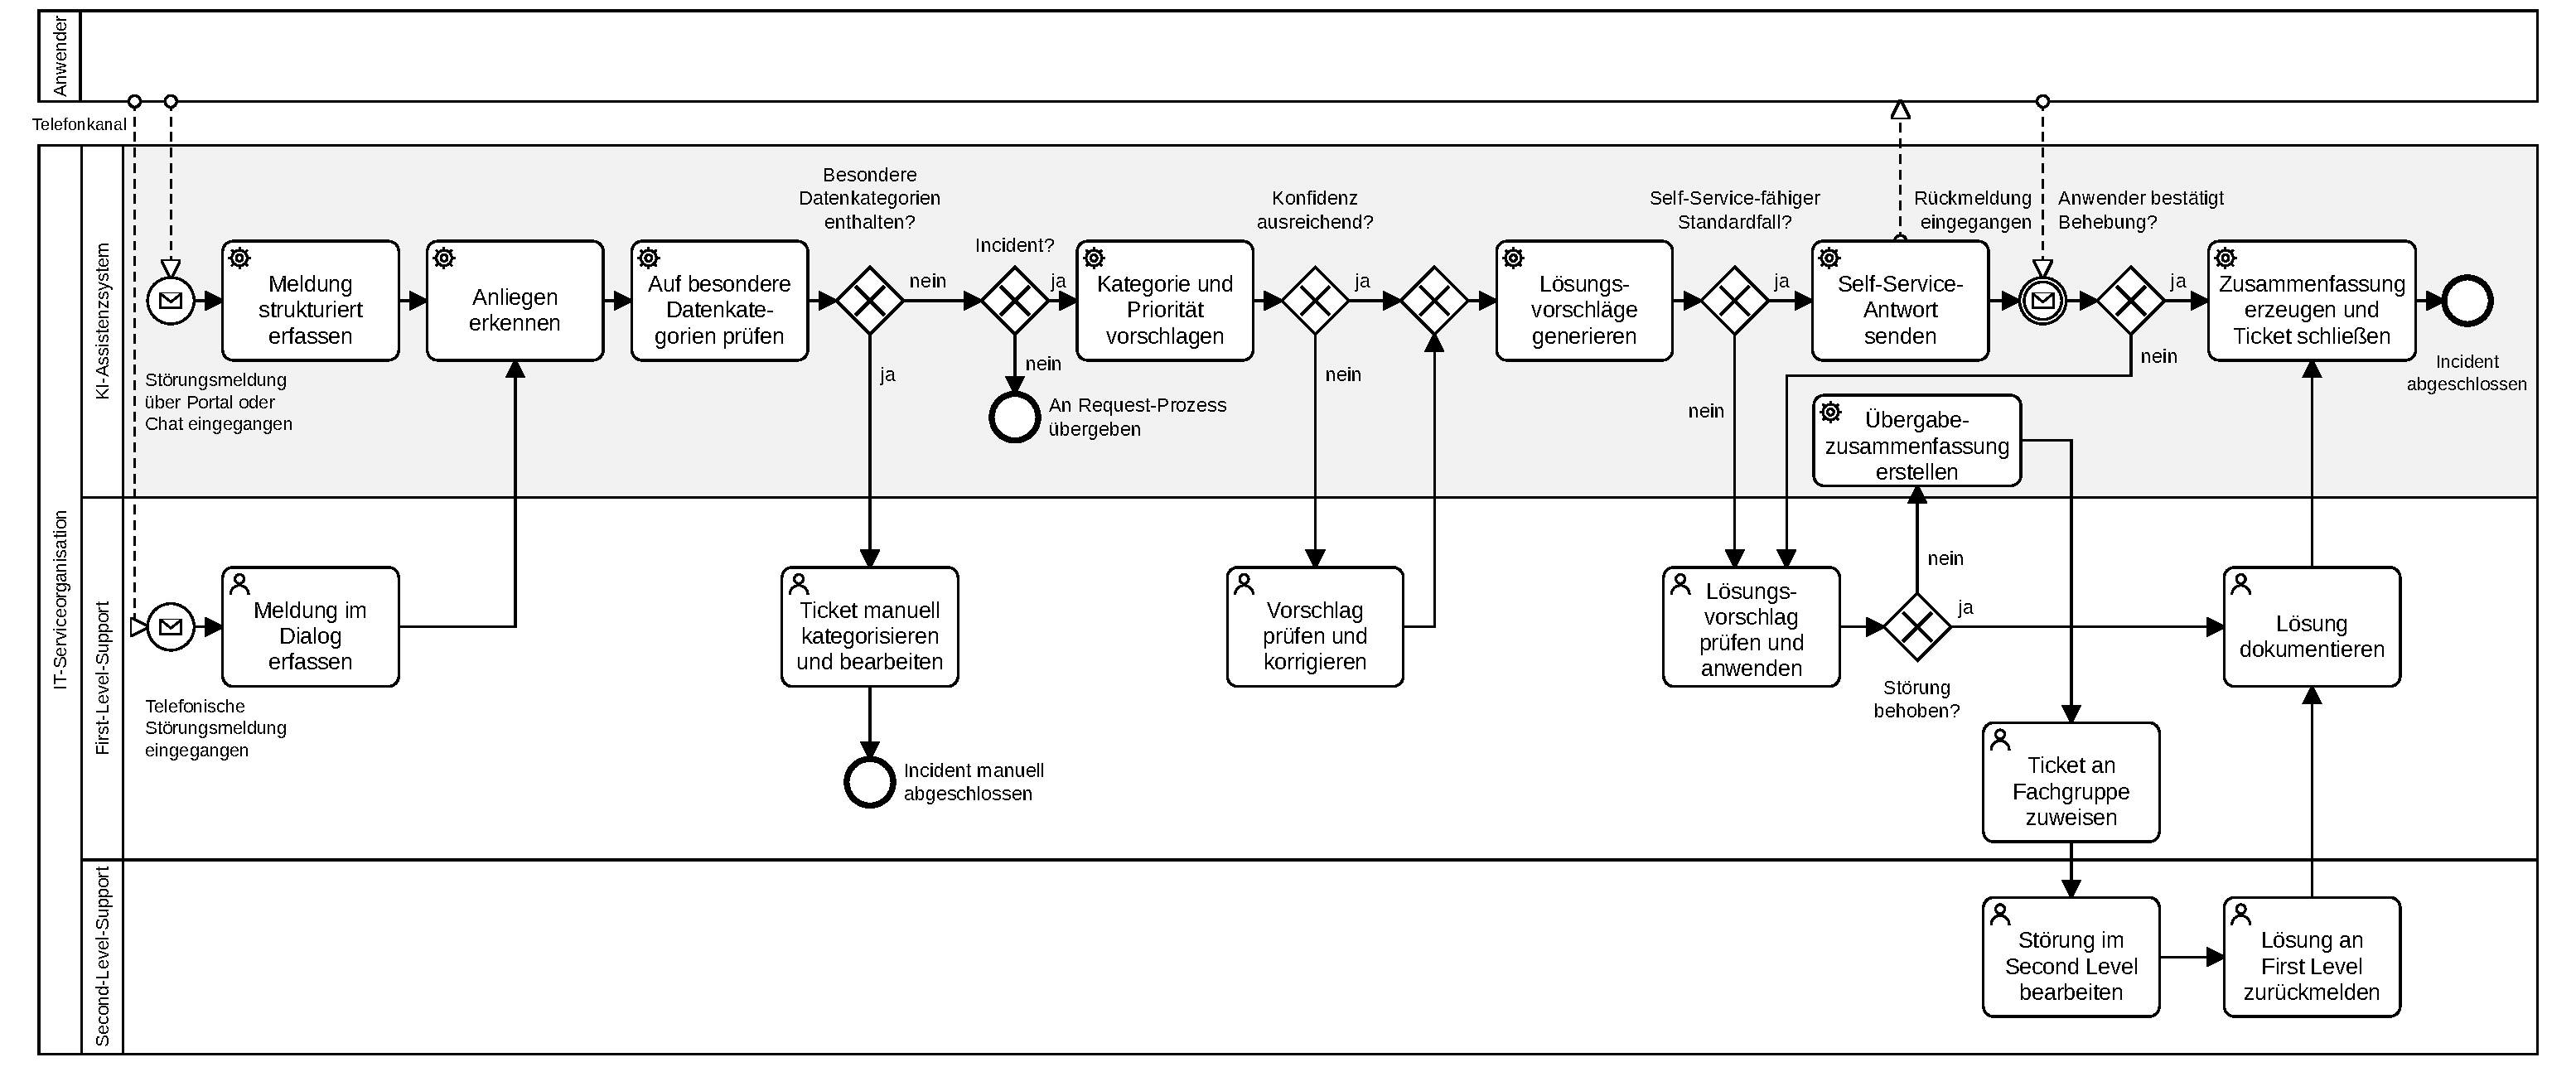
\includegraphics[width=\linewidth]{abb/abb7-bpmn-soll.pdf}
\end{figure}
\end{landscape}%
}

Meldungen \"uber Portal oder Chat l\"osen das Startereignis in der Lane des KI-Assistenzsystems aus, wo Erfassung und Anliegenerkennung maschinell ablaufen; die R\"uckfragen im Dialog erscheinen als Nachrichtenfl\"usse zum Pool des Anwenders. Vor der Anliegenweiche pr\"uft ein Service Task, ob der Freitext Angaben im Sinne des Art.~9 DSGVO enth\"alt. Da der Freitext zu diesem Zeitpunkt bereits die dialogorientierte Erfassung durchlaufen hat, setzt das Konzept voraus, dass diese Erfassung in einer kontrollierten Umgebung erfolgt, etwa durch einen intern betriebenen Dienst oder im Rahmen einer Auftragsverarbeitung, und dass die Eingaben nicht zum Training des Modells verwendet werden. Der Task beschr\"ankt sich auf die Feststellung, da bereits die Erkennung eine Verarbeitung darstellt, und leitet den Vorgang im Trefferfall ohne weitere maschinelle Bearbeitung an den Agenten; die inhaltlichen R\"uckfallkriterien aus Abschnitt~\ref{fallback} setzen damit vor allen \"ubrigen Entscheidungsknoten an. Der Agent bearbeitet einen solchen Vorgang vollst\"andig manuell nach dem Ablauf des Ist-Modells aus \autoref{fig:ist-prozess}; das Soll-Modell fasst diesen Teil im User Task \glqq Ticket manuell kategorisieren und bearbeiten\grqq{} zusammen und f\"uhrt ihn in ein eigenes Endereignis, sodass f\"ur diese Vorg\"ange weder die \"Ubergabe- noch die Abschlusszusammenfassung maschinell entsteht. Zwei Punkte bleiben dabei offen. Die Erkennung verarbeitet die betreffenden Angaben bereits und bedarf deshalb ihrerseits einer Grundlage nach Art.~9 Abs.~2 DSGVO; im Besch\"aftigungskontext kommt daf\"ur \S~26 Abs.~3 BDSG in Betracht, dessen Tragf\"ahigkeit im Einzelfall einer rechtlichen Pr\"ufung vorbehalten bleibt, die nicht Gegenstand dieser Arbeit ist.\footcites[Vgl.][Art.~9 Abs.~2]{DSGVO}[][\S~26 Abs.~3]{BDSG} Zudem kann die Erkennung eine Angabe \"ubersehen, sodass der Vorgang den automatisierten Pfad durchl\"auft. Der Entwurf begrenzt dieses Restrisiko, indem der Erfassungsdialog darauf hinweist, keine Gesundheits- oder vergleichbaren Angaben zu machen, und indem der Agent einen solchen Vorgang nachtr\"aglich kennzeichnen und damit aus der weiteren maschinellen Verarbeitung nehmen kann; ausschlie{\ss}en l\"asst es sich nicht. Anschlie{\ss}end trennt das Gateway \glqq Incident?\grqq{} St\"orungen von Service Requests, die den betrachteten Prozess \"uber ein eigenes Endereignis verlassen, da ihre Bearbeitung eigenen Regeln folgt. Diese Weiche ist die folgenreichste maschinelle Entscheidung des Modells, denn ein f\"alschlich ausgesteuerter Incident durchl\"auft keinen R\"uckweg und f\"allt erst im Request-Prozess auf. Der Entwurf entscheidet die Anliegenerkennung deshalb im Zweifel zugunsten des Incident-Pfades, da die irrt\"umliche Behandlung eines Service Requests als St\"orung lediglich Bearbeitungsaufwand erzeugt, w\"ahrend der umgekehrte Fehler eine St\"orung unbearbeitet lie{\ss}e. Als Service Request ausgesteuert wird eine Meldung nur, wenn sie einem im Request-Katalog hinterlegten Anliegen eindeutig entspricht; jede andere Meldung verbleibt im Incident-Pfad.

Telefonische Meldungen treten \"uber ein zweites Startereignis in der Lane des First-Level-Supports ein, wo der Agent die Erfassung im Dialog \"ubernimmt. Ab der Anliegenerkennung durchlaufen beide Kan\"ale denselben Pfad. Eine Ausnahme bildet der Self-Service, denn bei einer telefonischen Meldung spricht der Anwender bereits mit einem Agenten; sie gilt deshalb unabh\"angig vom Anliegen nicht als Self-Service-f\"ahiger Standardfall und nimmt stets den assistierten Pfad. Im \"Ubrigen liegt der Unterschied in der Erfassung, die beim Telefonkanal Agentenzeit bindet.

Auf dem Incident-Pfad entscheidet das Gateway \glqq Konfidenz ausreichend?\grqq{} \"uber die Behandlung des Kategorievorschlags; f\"ur die Priorit\"at gelten die inhaltlichen Kriterien aus Abschnitt~\ref{fallback}. Oberhalb des Schwellenwerts \"ubernimmt der Prozess den Vorschlag vorl\"aufig im Sinne des Human-on-the-Loop, unterhalb f\"uhrt der Pfad zum User Task \glqq Vorschlag pr\"ufen und korrigieren\grqq{}, dem ersten menschlichen Entscheidungsknoten des Modells.

Nach der Generierung der L\"osungsvorschl\"age trennt das Gateway \glqq Self-Service-f\"ahiger Standardfall?\grqq{} die vollautomatisierten von den assistierten Pfaden. Auf dem Ja-Pfad geht die Antwort unmittelbar an den Anwender, dessen R\"uckmeldung der Prozess \"uber ein Nachrichten-Zwischenereignis aufnimmt; best\"atigt er die Behebung, schlie{\ss}t das System den Vorgang mit einer Zusammenfassung ab, andernfalls \"ubernimmt der Agent. Bleibt die R\"uckmeldung innerhalb einer festzulegenden Frist aus, gilt die Behebung als nicht best\"atigt; auf ein eigenes Zeitereignis f\"ur diese Frist verzichtet das Modell zugunsten der Lesbarkeit. Auf dem assistierten Pfad pr\"uft der Agent den L\"osungsvorschlag, wendet ihn an und dokumentiert das Ergebnis, bevor der Vorgang maschinell abgeschlossen wird. Bleibt die St\"orung bestehen, leitet der Service Task \glqq \"Ubergabezusammenfassung erstellen\grqq{} die Eskalation ein, deren inhaltliche Anforderungen Abschnitt~\ref{kontexttransfer} behandelt; Bearbeitung im Second Level, R\"uckmeldung und Abschluss bleiben gegen\"uber dem Ist-Modell unver\"andert.

Der Vergleich beider Modelle zeigt eine Verschiebung der Arbeit. Die im Ist-Modell manuell ausgef\"uhrten vorgelagerten Tasks der Erfassung, Kategorisierung und Priorisierung sind f\"ur Meldungen \"uber Portal und Chat in die Lane des KI-Assistenzsystems gewandert; im Telefonkanal verbleibt die Erfassung beim Agenten. Von diesem Kanal abgesehen tritt der Agent nicht mehr am Anfang des Ablaufs in den Prozess ein, sondern an dessen Pr\"uf- und Entscheidungspunkten. Zugleich enth\"alt das Soll-Modell zwei Klassen von Pfaden, n\"amlich vollautomatisierte f\"ur risikoarme Standardf\"alle und assistierte f\"ur alle \"ubrigen Vorg\"ange.

\subsubsection{Definition der maschinellen und menschlichen Entscheidungsknoten}
\label{entscheidungsknoten}

Das Modell enth\"alt acht Stellen, an denen \"uber den weiteren Verlauf entschieden wird. Vier davon trifft das System, drei der Agent und eine der Anwender, der \"uber die Wirksamkeit der Self-Service-Antwort befindet und sich damit der Gestaltung durch die Organisation entzieht. Eine Sonderstellung nimmt die Pr\"ufung auf einen Self-Service-f\"ahigen Standardfall ein, weil sie dar\"uber befindet, ob \"uberhaupt ein Mensch mit dem Vorgang befasst wird. Die Eskalationsentscheidung bleibt umgekehrt auch dann menschlich, wenn die \"Ubergabezusammenfassung maschinell entsteht, da sie den Vorgang aus dem First Level heraus\-f\"uhrt und Kapazit\"at einer anderen Einheit bindet. \autoref{tab:entscheidungsknoten} fasst die Zuordnung samt der jeweils ausschlaggebenden Kriterien zusammen.

\begin{table}[!htb]
	\centering
	\caption{Entscheidungsknoten des Soll-Prozesses mit Zuordnung und Kriterium}
	\label{tab:entscheidungsknoten}
	\begin{tabularx}{\textwidth}{@{}p{4.6cm}p{2.1cm}X@{}}
		\toprule
		Entscheidungsknoten & Tr\"ager & Kriterium \\
		\midrule
		\glqq Besondere Datenkategorien enthalten?\grqq{} & maschinell & Erkennung von Angaben nach Art.~9 DSGVO; ein Treffer f\"uhrt in die vollst\"andig manuelle Bearbeitung mit eigenem Endereignis \\
		\glqq Incident?\grqq{} & maschinell & Ergebnis der Anliegenerkennung; Service Requests verlassen den Prozess \\
		\glqq Konfidenz ausreichend?\grqq{} & maschinell & Konfidenzwert des Kategorievorschlags gegen den Schwellenwert (Startwert 0,90, siehe Abschnitt~\ref{fallback}) \\
		\glqq Self-Service-f\"ahiger Standardfall?\grqq{} & maschinell & Zugeh\"origkeit zum festgelegten Katalog risikoarmer Standardf\"alle; telefonische Meldungen sind ausgenommen \\
		\glqq Vorschlag pr\"ufen und korrigieren\grqq{} & Agent & Konfidenz des Kategorievorschlags unterhalb des Schwellenwerts \\
		\glqq L\"osungsvorschlag pr\"ufen und anwenden\grqq{} & Agent & Vorgang au{\ss}erhalb des Standardfallkatalogs oder Eingriff in produktive Systeme \\
		\glqq Anwender best\"atigt Behebung?\grqq{} & Anwender & R\"uckmeldung des Anwenders auf die Self-Service-Antwort; bleibt sie aus, \"ubernimmt der Agent \\
		\glqq St\"orung behoben?\grqq{} & Agent & Bei erfolgloser Bearbeitung im First Level folgt die Eskalation; die Weitergabe bindet Kapazit\"at einer anderen Einheit \\
		\bottomrule
	\end{tabularx}
\end{table}

Die Zuordnung folgt einem einheitlichen Prinzip. Maschinell entschieden wird, was reversibel und risikoarm ist und dessen Fehlentscheidung im weiteren Verlauf noch bemerkt und korrigiert werden kann. Eine unzutreffend zugeordnete Kategorie f\"allt sp\"atestens bei der Bearbeitung auf und l\"asst sich ohne bleibenden Schaden \"andern. Eine Ausnahme bildet die Anliegenweiche, deren Fehlentscheidung nach Abschnitt~\ref{prozessarchitektur} keinen R\"uckweg kennt; der Entwurf sichert sie deshalb \"uber die dort beschriebene Entscheidungsregel zugunsten des Incident-Pfades ab. Anders verh\"alt es sich bei Entscheidungen, die den Vorgang beenden oder unmittelbar auf den Anwender wirken. Sie bleiben menschlich, soweit sie nicht dem definierten Katalog risikoarmer Standardf\"alle unterfallen. Darin liegt die prozessuale Umsetzung dessen, was Abschnitt~\ref{praemissen} aus Art.~22 DSGVO und den Anforderungen an die menschliche Aufsicht abgeleitet hat. Die Trennlinie verl\"auft damit nicht entlang des technischen K\"onnens der Modelle, sondern entlang der Tragweite der jeweiligen Entscheidung.

F\"ur die menschlichen Knoten gen\"ugt die blo{\ss}e Zuweisung allerdings nicht, da eine Pr\"ufung nur wirkt, wenn sie tats\"achlich m\"oglich ist. Aus den Leitlinien der Mensch-KI-Interaktion folgen daf\"ur drei Gestaltungsanforderungen.\footcite[Vgl.][S.~3]{Amershi2019} Der Vorschlag ist mit einer Konfidenzangabe zu versehen, damit der Agent einsch\"atzen kann, wie belastbar er ist. Die Begr\"undung des Vorschlags muss einsehbar sein, ohne dass der Agent das Bearbeitungsfenster verl\"asst. Die Korrektur schlie{\ss}lich darf nicht mehr Aufwand verursachen als die Best\"atigung, weil andernfalls der bequemere Weg stets in der \"Ubernahme l\"age. Die Protokollierung jeder Abweichung erg\"anzt diese Gestaltung, da sich an ihr ablesen l\"asst, ob eine Pr\"ufung \"uberhaupt stattfindet.

Zwei der maschinellen Knoten verlangen Kriterien, die bislang lediglich benannt sind. Sowohl der Schwellenwert der Konfidenzpr\"ufung als auch die Abgrenzung des Self-Service-f\"ahigen Standardfalls bestimmen, wie viel Automatisierung der Prozess tats\"achlich zul\"asst; beide entwickelt Abschnitt~\ref{eskalationSoll} im Rahmen des Eskalationsmanagements.

\subsection{Eskalationsmanagement im Soll-Prozess}
\label{eskalationSoll}

Der Begriff der Eskalation erh\"alt im Soll-Prozess eine doppelte Bedeutung. Neben die aus Abschnitt~\ref{eskalationIst} bekannte Weitergabe vom First an den Second Level tritt der R\"uckfall von der maschinellen auf die menschliche Bearbeitung. Abschnitt~\ref{fallback} entwickelt die Kriterien dieses Fallbacks, Abschnitt~\ref{kontexttransfer} die \"Ubergabe an den Second-Level-Support.

\subsubsection{Kriterien für den automatisierten Fallback zum menschlichen Bearbeiter}
\label{fallback}

Der R\"uckfall auf den menschlichen Pfad ist regul\"arer Bestandteil des Entwurfs und kein Fehlerfall. Ein System, das jeden Vorgang selbst zu Ende bearbeitet, w\"are lediglich weniger zur\"uckhaltend, aber nicht leistungsf\"ahiger. Die eigentliche Anforderung besteht darin, dass das System erkennt, wann es nicht entscheiden sollte, und den Vorgang abgibt, bevor eine Fehlentscheidung wirksam wird. Die Kriterien daf\"ur lassen sich in konfidenzbasierte und inhaltliche trennen.

Das erste Kriterium kn\"upft an den Konfidenzwert eines Vorschlags an. Unterschreitet er den Schwellenwert, f\"uhrt das Gateway \glqq Konfidenz ausreichend?\grqq{} den Schritt dem Agenten zu. Das Kriterium bezieht sich allein auf den Kategorievorschlag, denn nur das in Abschnitt~\ref{kategorisierungSoll} vorgesehene Encoder-Modell gibt einen Wert aus, der sich als Sicherheit einer Klassifikation deuten l\"asst; die Priorit\"at wird regelbasiert aus den extrahierten Indikatoren abgeleitet, und die Unsicherheit ihrer Extraktion fangen die nachstehenden inhaltlichen Kriterien und die Pr\"ufung durch den Agenten auf. Die Konstruktion tr\"agt allerdings nur, soweit der ausgegebene Wert die tats\"achliche Trefferwahrscheinlichkeit widerspiegelt. Guo et al.~zeigen, dass moderne neuronale Netze systematisch \"uberkonfident seien und ihre Ausgabewerte ohne Kalibrierung nicht als Wahrscheinlichkeiten interpretiert werden d\"urften.\footcite[Vgl.][hier S.~1322]{Guo2017} Vor Inbetriebnahme ist das Modell deshalb zu kalibrieren, und die Schwelle ist laufend an der Korrekturquote der Agenten zu \"uberpr\"ufen, da h\"aufige Korrekturen oberhalb der Schwelle anzeigen, dass sie zu niedrig liegt. Der Entwurf setzt die Schwelle bei einem Konfidenzwert von 0,90 an. Dieser Wert ist keine empirisch ermittelte Gr\"o{\ss}e, sondern eine Entwurfsentscheidung f\"ur den Pilotbetrieb, in dem die G\"ute der Kalibrierung noch nicht belegt ist; solange offenbleibt, wie weit die ausgegebenen Werte die Trefferwahrscheinlichkeit wiedergeben, muss die Schwelle oberhalb dessen liegen, was bei nachgewiesen kalibrierten Werten gen\"ugte. F\"ur einen hohen Startwert spricht zudem die ungleiche Fehlerwirkung, denn eine zu hohe Schwelle f\"uhrt dem Agenten lediglich Vorg\"ange zu, die er ohnehin bearbeitet h\"atte, w\"ahrend eine zu niedrige fehlerhafte Zuordnungen unbemerkt in den Prozess tr\"agt. Schlie{\ss}lich entspricht ein hoher Startwert dem in Abschnitt~\ref{voraussetzungen} begr\"undeten stufenweisen Vorgehen, da sich die Schwelle mit belegter Vorschlagsqualit\"at schrittweise absenken l\"asst, statt sie nachtr\"aglich anheben zu m\"ussen. Sie ist im Rahmen der in Abschnitt~\ref{herausforderungen} er\"orterten Grenzen zu \"uberpr\"ufen. Wie viele Vorschl\"age unterhalb der Schwelle bleiben und damit vom Agenten zu pr\"ufen sind, h\"angt von Modell und Ticketbestand ab und l\"asst sich vorab nicht angeben; die Simulation in Abschnitt~\ref{simulation} setzt diesen Anteil im mittleren Szenario mit 35~Prozent an und variiert ihn zwischen 20 und 55~Prozent.

Unabh\"angig von der Konfidenz greifen inhaltliche Kriterien. Am Anfang steht die in Abschnitt~\ref{prozessarchitektur} beschriebene Pr\"ufung auf besondere Kategorien personenbezogener Daten, die im Trefferfall jede weitere automatisierte Bearbeitung beendet. Der in Abschnitt~\ref{incidentProzess} abgegrenzte Major-Incident-Prozess bleibt auch hier ausgenommen und tritt allein als Abbruchkriterium des automatisierten Ablaufs auf. Dem Agenten zugef\"uhrt wird ein Vorgang daher dann, wenn die bei der Erfassung gewonnenen Indikatoren auf einen Major Incident hindeuten, etwa weil mehrere Meldungen denselben Dienst betreffen oder die Schilderung einen gro{\ss}fl\"achigen Ausfall nahelegt. Ma{\ss}geblich sind dabei die Angaben des Melders und nicht die vom System vorgeschlagene Priorit\"at, da diese erst aus dem Schritt hervorgeht, den das Kriterium aussetzen soll. Scheitert derselbe Anwender wiederholt mit demselben Anliegen im Self-Service, f\"uhrt der Prozess den Fall ebenfalls dem Agenten zu, statt eine weitere Antwort zu erzeugen. Schlie{\ss}lich gen\"ugt der ausdr\"uckliche Wunsch nach menschlicher Bearbeitung. Die drei zuletzt genannten Kriterien, also der Hinweis auf einen Major Incident, das wiederholte Scheitern im Self-Service und der Wunsch nach menschlicher Bearbeitung, k\"onnen an jeder Stelle des automatisierten Ablaufs eintreten und sind in \autoref{fig:soll-prozess} deshalb nicht als eigene Gateways dargestellt; sie er\"offnen keinen zus\"atzlichen Pfad, sondern m\"unden jeweils in die Bearbeitung durch den Agenten. Der in Abschnitt~\ref{loesungsvorschlaege} genannte Katalog ist dabei als Positivliste ausgestaltet, sodass jeder nicht ausdr\"ucklich aufgenommene Fall ohne weitere Pr\"ufung beim Agenten landet. Aufgenommen wird ein Anliegen nur, wenn mehrere Bedingungen zugleich erf\"ullt sind. Seine L\"osung ist in einem gepr\"uften Wissensartikel dokumentiert und vom Anwender selbst ausf\"uhrbar, sie greift weder in produktive Systeme noch in Berechtigungen ein und l\"asst sich ohne bleibenden Schaden r\"uckg\"angig machen, wie es dem Zuordnungsprinzip aus Abschnitt~\ref{entscheidungsknoten} entspricht. \"Uber die Aufnahme entscheidet der Prozessverantwortliche, und ein Anliegen verl\"asst den Katalog wieder, sobald Anwender es auff\"allig h\"aufig nicht \"uber den Self-Service l\"osen. Diese Konstruktion verschiebt die Begr\"undungslast vom R\"uckfall auf die Vollautomatisierung.

Der Fallback wirkt allerdings nur, soweit der Mensch die maschinelle Vorarbeit tats\"achlich korrigiert. Green und Chen untersuchen Entscheidungen, bei denen Personen algorithmische Vorhersagen einbeziehen, und stellen fest, dass diese die Vorhersagen schlecht kalibriert nutzten; sie folgten ihnen teils auch dann, wenn sie unzutreffend seien, und erkannten deren Fehler nicht zuverl\"assig.\footcite[Vgl.][hier S.~1]{GreenChen2019} Der Entwurf zieht daraus zwei Folgerungen. Der Fallback h\"alt den Vorgang an, bis der Agent die Kategorie selbst festgelegt hat; der Vorschlag wird nicht vorl\"aufig \"ubernommen, sondern ausdr\"ucklich als unsicher gekennzeichnet. Zudem macht die in Abschnitt~\ref{entscheidungsknoten} geforderte Konfidenzanzeige die Unsicherheit sichtbar, anstatt sie hinter einer scheinbar fertigen Antwort verschwinden zu lassen. Beides beseitigt das Problem nicht, begrenzt aber die Wahrscheinlichkeit, dass ein unsicherer Vorschlag unbemerkt durchl\"auft.

\subsubsection{Übergabe und Kontexttransfer an den Second-Level-Support}
\label{kontexttransfer}

Die Abschnitte~\ref{eskalationIst} und \ref{unstrukturiert} haben gezeigt, dass eine l\"uckenhafte Dokumentation beim \"Ubergang in den Second Level Doppelarbeit erzeugt, weil R\"uckfragen erforderlich werden und Teile der Diagnose erneut durchlaufen werden. An dieser Stelle setzt der Service Task \glqq \"Ubergabezusammenfassung erstellen\grqq{} aus Abschnitt~\ref{prozessarchitektur} an. Er bereitet den Kontext auf, bevor die Zuweisung an die Fachgruppe erfolgt, und macht die Qualit\"at der \"Ubergabe damit unabh\"angig davon, wie viel Zeit dem einzelnen Agenten daf\"ur bleibt.

Der \"ubergebene Kontext besteht aus vier Bestandteilen. Die bei der Erfassung gewonnenen strukturierten Ticketdaten liefern den Ausgangszustand. Hinzu treten die gepr\"uften L\"osungshypothesen samt ihrem Ergebnis, wobei gerade die verworfenen Ans\"atze den Wert ausmachen, da sie dem Second Level ersparen, denselben Weg noch einmal zu gehen. Weiter werden die vom Abrufsystem herangezogenen Wissensartikel mit ihren Fundstellen ausgewiesen. Den vierten Bestandteil bildet eine maschinell erzeugte Verlaufszusammenfassung, die l\"angere Dialoghistorien auf das Entscheidungsrelevante verdichtet und dabei die in Abschnitt~\ref{llmFunktion} beschriebene Zusammenfassungsf\"ahigkeit nutzt. Chen et al.~zeigen f\"ur die Ursachenanalyse von Cloud-Incidents, dass automatisch gesammelter und verdichteter Diagnosekontext die nachgelagerte Bearbeitung unterst\"utzen k\"onne.\footcite[Vgl.][hier S.~674\,f.]{Chen2024}

Die Zusammenfassung ist selbst ein generiertes Artefakt und damit fehleranf\"allig. Der Entwurf sieht deshalb vor, dass die vollst\"andige Rohhistorie aus Dialog, ausgef\"uhrten Systemschritten und Konfidenzwerten im Ticket einsehbar bleibt. Die Zusammenfassung erg\"anzt diese Historie und tritt nicht an ihre Stelle, sodass der Bearbeiter im Zweifel auf die urspr\"ungliche Fassung zur\"uckgreifen kann. Die durchgehende Protokollierung der maschinellen Schritte erf\"ullt zugleich die in Abschnitt~\ref{voraussetzungen} begr\"undete Anforderung an die Nachvollziehbarkeit. Ob das so entwickelte Konzept die in Abschnitt~\ref{kennzahlen} benannten Kennzahlen zu verbessern verspricht und welche Grenzen ihm gesetzt sind, pr\"uft Kapitel~\ref{evaluation}.

